\chapter{Floating point arithmetic}%
\label{cha:rounding_errors}
\minitoc

\section*{Introduction}%
\label{sec:introduction}
% In numerical simulation,
% errors arise from four distinct sources:
% \begin{itemize}
%     \item
%         The \emph{modeling error} accounts for the mismatch between reality and the mathematical equations describing it.
%         Mathematical equations are generally only an approximation of reality.
%     \item
%         The \emph{numerical error}
%         refers to the error introduced by numerical methods,
%         which are generally not exact;
%         they only provide approximate solutions to the mathematical equations.
%     \item
%         The \emph{roundoff errors} come from the fact that
%         computers are unable to store the majority of real numbers exactly.
%         The number $\pi$, for example,
%         contains an infinite amount of digits
% \end{itemize}

When we study numerical algorithms in the next chapters,
we assume implicitly that the operations involved are performed exactly.
On a computer, however, only a subset of the real numbers can be stored and,
consequently, many arithmetic operations are performed only approximately.
This is the source of the so-called \emph{round-off errors}.
% Whether or not these inevitable errors are sufficiently small to be neglected in a numerical method
% depends in general on the \emph{numerical stability} of the method.
% A numerical method is said to be \emph{numerically unstable} is small errors are magnified,
% and \emph{numerically stable} otherwise.
% these errors generally need not be a cause worry when they appear in methods that are numerically stables.
The rest of this chapter is organized as follows.
\begin{itemize}
    \item
        In \cref{sec:binary_representation_of_real_numbers},
        we briefly discuss the binary representation of real numbers.
    \item
        In \cref{sec:set_of_values},
        we describe the set of floating point numbers that can be represented in the usual floating point formats;
    \item
        In \cref{sec:arithmetic_operations_between_floating_point_formats}
        we explain how arithmetic operations between floating point numbers behave.
        We insist in particular on the fact that,
        in a calculation involving several successive arithmetic operations,
        the result of each intermediate operation is stored as a floating point number,
        with a possible error.
        % This is why \texttt{1.0 + 1e-100 - 1.0} returns \texttt{0.0},
        % in the usual double-precision format.
    \item
        In \cref{sec:encoding_of_floating_point_numbers},
        we briefly present how floating point numbers are encoded
        according to the IEEE 754 standard, widely accepted today.
        We discuss also the encoding of special values such as \texttt{Inf}, \texttt{-Inf} and \texttt{NaN}.
\end{itemize}
In order to completely describe a floating-point system,
one would in principle need to also discuss the storage of integer numbers
and the conversion mechanisms between different number formats,
as well as a number of edge cases.
For instance, the reference IEEE 754 standard specifies that \texttt{NaN == NaN} must evaluate to \texttt{false},
which is somewhat arbitrary but may be useful in some situations.
Needless to say,
a comprehensive discussion of the subject is beyond the scope of this course;
our aim in this chapter is only to introduce the key concepts.

\section{Binary representation of real numbers}%
\label{sec:binary_representation_of_real_numbers}

Given any integer number $\beta > 0$, called the \emph{base},
a real number $x$ can always be expressed as a finite or infinite series of the form
\begin{equation}
    \label{eq:base_representation}
    x = (-1)^s \sum_{k=-n}^{\infty} a_k \beta^{-k}, \qquad 0 \leq a_k < \beta.
\end{equation}
The number $x$ may then be denoted as $(-1)^s (a_{-n} a_{-n+1}\dots a_{-1} a_{0}.a_{1} a_{2} \dots)_{\beta}$,
where the subscript $\beta$ indicates the base and $s \in \{0, 1\}$ encodes the sign.
This numeral system is called the \emph{positional notation} and is universally used today,
both by humans (usually with $\beta=10$) and machines (usually with $\beta=2$).
If the base~$\beta$ is omitted,
it is always assumed that $\beta = 10$ unless otherwise specified
-- this is the \emph{decimal} representation.
% It is likely that the prevalence of base 10 in human writing is a consequence of human morphology,
% although this fact has not been demonstrated by historians.
In computer science, several bases other than 10 are regularly employed,
for example the following:
\begin{itemize}
    \item
        Base 2 (binary) is the usual choice for storing numbers on a machine.
        The binary format is convenient because the digits have only two possible values, 0 or 1,
        and so they can be stored using simple electrical circuits with two states.
        We employ the binary notation extensively in the rest of this chapter.
        Notice that, just like multiplying and dividing by~10 is easy in base 10,
        multiplying and dividing by 2 is very simple in base 2:
        these operations amount to shifting all the bits by one position to the left or right,
        respectively.

    \item
        Base 16 (hexadecimal) is sometimes convenient to represent numbers in a compact manner.
        In order to represent the values 0-15 by a single digit,
        16 different symbols are required, which are conventionally denoted by $\{0,1,2,3,4,5,6,7,8,9,A,B,C,D,E,F\}$.
        With this notation, we have $(FF)_{16} = (255)_{10}$, for example.

        The hexadecimal notation is often used in programming languages for describing colors specified by a triplet $(r,g,b)$ of values between 0 and 255,
        corresponding to the primary colors \emph{red}, \emph{blue} and \emph{green}.
        Since the number of possible values for the components is $256 = 16^2$,
        only 2 digits are required to represent these in the hexadecimal notation.
        Hexadecimal numbers are also employed in IPv6 addresses.
\end{itemize}

\subsection{Conversion between binary and decimal formats}%
Obtaining the decimal representation of a binary number can be achieved from~\eqref{eq:base_representation},
using the decimal representations of the powers of 2.
Since all the positive and negative powers of 2 have finite decimal representations,
any real number with a finite representation in base 2 has a finite representation also in base 10.
For example, $(0.01)_2 = (0.25)_{10}$ and $(0.111)_2 = 0.875$.
\begin{example}
    [Converting a binary number to decimal notation]
    \label{example:converting_binary_to_decimal}
    Let us calculate the decimal representation of $x = (0.\overline{10})_2$,
    where the horizontal line indicates repetition: $x = (0.101010\dots)_2$.
    By definition, it holds that
    \[
        x = \sum_{k=0}^{\infty} a_k 2^{-k},
    \]
    where $a_k = 0$ if $k$ is even and 1 otherwise.
    Thus, the series may be rewritten as
    \[
        x = \sum_{k=0}^{\infty} 2^{-(2k+1)} = \frac{1}{2} \sum_{k=0}^{\infty} (2^{-2})^k.
    \]
    We recognize on the right-hand side a geometric series with common ratio $r = 2^{-2} = \frac{1}{4}$,
    and so we obtain
    \[
        x = \frac{1}{2} \left( \frac{1}{1-r} \right) = \frac{2}{3} = 0.\overline 6.
    \]
\end{example}

Obtaining the binary representation of a decimal number may prove more difficult,
because negative powers of 10 have \emph{infinite} binary representations,
as the example below demonstrates.
There is, however, a simple procedure to perform the conversion,
which we present for the specific case of a real number $x$ with decimal representation of the form $x = (0.a_1\dots a_n)_{10}$.
In this setting,
the bits~$(b_1, b_2, \dots)$ in the binary representation of $x = (0.b_1b_2b_2 \dots)_2$ may be obtained as follows:
\begin{algorithm}
\caption{Conversion of a number to binary format}%
\label{algo:conversion_to_binary}%
\begin{algorithmic}[1]
\State $i \gets 1$
\While{$x \neq 0$}
    \State $x \gets 2x$%
    \label{line:after_while}
    \If{$x \geq 1$}
        \State $b_i \gets 1$
    \Else
        \State $b_i \gets 0$
    \EndIf
    \State $x \gets x - b_i 2^{-i}$
    \State $i \gets i+1$
\EndWhile
\end{algorithmic}
\end{algorithm}

\begin{example}
    [Converting a decimal number to binary notation]
    Let us calculate the binary representation of $x = \frac{1}{3} = (0.\overline{3})_{10}$.
    We apply~\cref{algo:conversion_to_binary} and collate the values of $i$ and $x$ at the beginning of each iteration,
    i.e.\ just before~\cref{line:after_while}, in the table below.
    \begin{center}
    \begin{tabular}{|c|c|c|}
        \hline
        $i$ & $x$ & Result \\ \hline
        $1$ & $\frac{1}{3}$ & 0.\textbf{0}000\dots \\ \hline
        $2$ & $\frac{2}{3}$ & 0.0\textbf{1}00\dots \\ \hline
        $3$ & $\frac{1}{3}$ & 0.00\textbf{0}0\dots \\ \hline
    \end{tabular}
    \end{center}
    Since $x$ in the last row is again $\frac{1}{3}$,
    successive bits alternate between 0 and 1,
    and the binary representation of $x$ is given by $(0.\overline{01})_2$.
    This is not surprising since $2x = (0.66)_{10} = (0.\overline{10})_2$,
    as we saw in~\cref{example:converting_binary_to_decimal}.
\end{example}

\subsection{Exercises}%

\begin{exercise}
    \label{exercise:non_unique_representation}
    Show that if a number $x \in \real$ admits a finite representation~\eqref{eq:base_representation} in base $\beta$,
    then it also admits an infinite representation.
    \textbf{Hint:} You may have learned before that $(0.\overline 9)_{10} = 1$.
\end{exercise}

\begin{exercise}
    How many digits does it take to represent all the integers from 0 to $10^{10} - 1$ in decimal and binary format?
    What about the hexadecimal format?
\end{exercise}

\begin{exercise}
    Find the decimal representation of $(0.000\overline{1100})_2$.
\end{exercise}

\begin{exercise}
    Find the binary representation of $(0.1)_{10}$.
\end{exercise}

\begin{exercise}
    Implement~\cref{algo:conversion_to_binary} on a computer and verify that it works.
    Your function should take as argument an array of integers containing the digits after the decimal point,
    that is an array of the form \verb?[a_1, ..., a_n]?.
\end{exercise}

\begin{exercise}
    As mentioned above, \cref{algo:conversion_to_binary} works only for decimal numbers of the specific form~$x = (0.a_1\dots a_n)_{10}$.
    Find and implement a similar algorithm for integer numbers of the form $x = (a_{-n} \dots a_{0})_{10}$.
\end{exercise}

\section{Set of values representable in floating point formats}%
\label{sec:set_of_values}
We mentioned in the introduction that,
because of memory limitations,
only a subset of the real numbers can be stored exactly in a computer.
Nowadays, the vast majority of programming languages and software comply with the IEEE 754 standard,
which requires that the set of representable numbers be of the form
\begin{align}
    \notag
    \floating (p, E_{\min}, E_{\max})
    = \Bigl\{ & (-1)^s 2^E (b_0. b_1 b_2 \dots b_{p-1})_2 \colon \\
    \label{eq:number_format}%
              & \qquad s \in \{0, 1\}, b_i \in \{0, 1\} \, \text{and} \, E_{\min} \leq E \leq E_{\max} \Bigr\}.
\end{align}
In addition to these, floating number formats provide the special entities \texttt{Inf}, \texttt{-Inf} and \texttt{NaN},
the latter being an abbreviation for \emph{Not a Number}.
Three parameters appear in the set definition~\eqref{eq:number_format}.
The parameter $p \in \nat_{>0}$ is the number of significant bits (also called the precision),
and $(E_{\min}, E_{\max}) \in \integer^2$ are respectively the minimum and maximum exponents.
From the precision, the \emph{machine epsilon} is defined as $\varepsilon_{M} = 2^{-p-1}$;
its significance is discussed in~\cref{sub:relative_error_and_epsilon_machine}.

For a number $x \in \floating(p, E_{\min}, E_{\max})$,
$s$ is called the \emph{sign}, $E$ is the \emph{exponent} and
$b_0. b_1 b_2 \dots b_{p-1}$ is the \emph{significand}.
The latter can be divided into a \emph{leading bit} $b_0$ and the fraction $b_1 b_2 \dots b_{p-1}$,
to the right of the binary point.
The most widely used floating point formats are the \emph{single} and \emph{double precision} formats,
which are called respectively \texttt{Float32} and \texttt{Float64} in Julia.
Their parameters are summarized in~\cref{table:floating_point_formats},
and in the rest of this section we use the shorthand notation $\floating_{32}$ and $\floating_{64}$.
\begin{table}[ht]
    \centering
    \begin{tabular}{|c|c|c|c|}
        \hline
        & Half precision & Single precision & Double precision
        \\ \hline
        $p$ & 11 & 24 & 53
        \\ \hline
        $E_{\min}$ & -14 & -126 & -1022
        \\ \hline
        $E_{\max}$ & 15 & 127 & 1023
        \\ \hline
    \end{tabular}
    \caption{%
        Floating point formats.
        The first column corresponds to the lesser known \emph{half-precision} format.
        This format,
        which is available through the \texttt{Float16} type in Julia,
        is more recent than the single and double precision formats.
        It was introduced in the 2008 revision to the IEEE 754 standard of 1985,
        a revision known as IEEE 754-2008.
    }%
    \label{table:floating_point_formats}
\end{table}

\begin{remark}
    Some definitions,
    notably that in~\cite[Section 2.5.2]{MR2265914},
    include the base~$\beta$
    as an additional parameter in the definition of the number format~\eqref{eq:number_format}.
    Since the binary format ($\beta = 2$) is always employed in practice,
    we focus on this case for simplicity in most of this chapter.
\end{remark}

\subsection{Make the floating point representation unique}%
\label{sub:defining_a_unique_representation}

Given a real number $x \in \floating (p, E_{\min}, E_{\max})$,
the exponent $E$ and significand  are generally not uniquely defined.
For example, the number $2.0 \in \floating_{64}$ may be expressed as $(-1)^0 2^1 (1.00\dots00)_2$ or equivalently as $(-1)^0 2^{2} (0.100\dots00)_2$.
To remove this ambiguity,
one may define the \emph{standard representation} of a number by requiring that
\begin{itemize}
    \item either $E > E_{\min}$ and $b_0 = 1$;
    \item or $E = E_{\min}$, in which case the leading bit may be 0.
\end{itemize}
One may prove that these rules define the exponent and significand uniquely.
\begin{proposition}
    \label{prop:uniqueness_standard_representation}
    Assume that
    \begin{equation}
        \label{eq:equality_floating_point}
        x = (-1)^s (2^{E} b_0.b_1\dots b_{p-1})_2 = (-1)^{\widetilde s} (2^{\widetilde E} \widetilde b_0. \widetilde b_1\dots \widetilde b_{p-1})_2,
    \end{equation}
    where the parameter sets $(s, E, b_0, \dots b_{p-1})$ and $(\widetilde s, \widetilde E, \widetilde b_0, \dots, \widetilde b_{p-1})$ both satisfy the above rule.
    Then $E = \widetilde E$ and $b_i = \widetilde b_i$ for $i \in \{0, \dots, p-1\}$.
\end{proposition}
\begin{proof}
    We show that $E = \widetilde E$,
    after which the equality of significands follows trivially,
    Let us assume for contradiction that $E > \widetilde E$
    and denote the left and right-hand side of~\eqref{eq:equality_floating_point} by~$x$ and~$\widetilde x$, respectively.
    Then~$E > E_{\min}$, implying that $b_0 = 1$ and so $2^{E} \leq |x| < 2^{E+1}$.
    On the other hand, it holds that $|\widetilde x| < 2^{\widetilde E+1}$ regardless of whether $\widetilde E = E_{\min}$ or not.
    Since $E \geq \widetilde E + 1$ by assumption,
    we deduce that $|\widetilde x| < 2^E \leq |x|$,
    which contradicts the equality $x = \widetilde x$.
\end{proof}

In view of \cref{prop:uniqueness_standard_representation},
we can talk without ambiguity about \emph{the} exponent or \emph{the} significand of a number in $\floating (p, E_{\min}, E_{\max})$.
A floating point number whose standard representation has a leading bit equal to 1 is called \emph{normalized},
whereas one with a leading bit equal to zero is called \emph{subnormal} or \emph{denormalized}.
We give more information on this subject in~\cref{sec:encoding_of_floating_point_numbers},
which is devoted specifically to the encoding of floating point numbers.

% In a computer, however, each number in a floating point format is always represented in the same manner,
% which is useful in order to perform comparisons:
% since the representation is unique,
% two numbers are equal if only if their sign, exponent and significand are equal.

\begin{remark}
    [Nonuniqueness of the floating point represention of 0.0]
    The sign $s$ is clearly unique for any number in a floating point format,
    except for $0.0$,
    which could in principle be represented as
    \[
        (-1)^0 2^{E_{\min}} (0.00\dots00)_2
        \qquad \text{or} \qquad
        (-1)^1 2^{E_{\min}} (0.00\dots00)_2.
    \]
    In practice, both representations of 0.0 are available on most machines,
    and these behave slightly differently.
    For example $\texttt{1/(0.0) = Inf}$ but $\texttt{1/(-0.0) = -Inf}$.
\end{remark}

In \texttt{Julia}, non-integer numbers are interpreted as \texttt{Float64} by default,
which you may verify by using the \texttt{typeof} function.
In order to define a number of type \texttt{Float32},
the suffix $\texttt{f0}$ must be appended to the decimal expansion.
For instance, the command $\texttt{a = 4.0f0}$ defines a floating point number~\texttt{a} of type \texttt{Float64}.


\subsection{Relative error and epsilon machine}%
\label{sub:relative_error_and_epsilon_machine}
Let $x$ be a nonzero real number and $\widehat x$ be an approximation.
We define the absolute and relative errors of the approximation as follows.
\begin{definition}
    [Absolute and relative error]
    The absolute error is given by $|x - \widehat x|$,
    whereas the relative error is
    \[
        \frac{|x - \widehat x|}{|x|}
    \]
\end{definition}

The following establishes a link between the machine $\varepsilon_M$ and
the relative error between a real number and the closest member of a floating point format.
\begin{proposition}
    \label{prop:relative_error_and_machine_epsilon}
    Let $x_{\min}$ and $x_{\max}$ denote the smallest and largest \emph{normalized} positive numbers in a format $F = \floating(p, E_{\min}, E_{\max})$.
    If $x \in [-x_{\max}, -x_{\min}] \cup [x_{\min}, \leq x_{\max}]$,
    then there exists $\widehat x \in \floating(p, E_{\min}, E_{\max})$ such that
    \begin{equation}
        \label{eq:bound_epsilon_machine}
        \min_{\widehat x \in F} \frac{|x - \widehat x|}{|x|} \leq \frac{1}{2} 2^{-(p-1)}
        \leq \frac{1}{2} \varepsilon_M.
    \end{equation}
\end{proposition}
\begin{proof}
    For simplicity, we also assume that $x > 0$.
    Let us introduce $n = \lfloor \log_2(x) \rfloor$ and $y := 2^{-n} x$.
    Since $y \in [1, 2)$,
    it has a binary representation of the form
    \(
        (1.b_1 b_2\dots)_2,
    \)
    where the bits after the binary point are not all equal to 1 ad infinitum.
    Thus
    \(
        x = 2^{n} (1.b_1 b_2\dots)_2,
    \)
    and from the assumption that $x_{\min} \leq x \leq x_{\max}$
    we deduce hat $E_{\min} \leq n \leq E_{\max}$.
    % \footnote{%
    %     The inequality here is strict,
    %     because $2^{E_{\min} - 1} (1.\overline{1})_2 = 2^{E_{\min}} = x_{\min}$.
    %     Remember that the binary expansion of a real number is generally not unique!
    %     See~\cref{exercise:non_unique_representation}.
    % }
    % which is excluded by assumption.
    Then we define the truncated number $x_- \in F$ by truncating the binary expansion of $x$ as follows:
    \[
        x_- = 2^n (1.b_1 \dots b_{p-1})_2.
    \]
    The distance between $x_-$ and its successor in $F$,
    which we denote by $x_+$, is given by $2^{n-p+1}$.
    Consequently, it holds that
    \[
        (x_+ - x) + (x-x_-) = x_+ - x_- = 2^{n-p+1}.
    \]
    Clearly, since both summands on the left-hand side are positive,
    this implies that either $x_+ - x$ or $x - x_-$ is bounded from above by $\frac{1}{2} 2^{n-p+1} \leq \frac{1}{2} 2^{-p+1}x$,
    which concludes the proof.
\end{proof}

The machine epsilon can be viewed as the maximum relative difference between a normalized floating point number $x$ and its successor,
defined as the smallest number in the floating point format that is strictly larger than $x$.
\Cref{fig:float64_density} depicts the density of double-precision floating point numbers.
The figure shows that, as the absolute value increases,
the density of floating point number decreases.
We also notice that the density is piecewise constant with discontinuities at powers of 2,
which correspond to a change of exponent.
\Cref{fig:float64_spacing} illustrates the relative spacing between successive floating point numbers,
in units of machine precision.
Although the absolute spacing increases with the absolute value of $x$,
the relative spacing oscillates between~$\frac{1}{2} \varepsilon_{M}$ and~$\varepsilon_M$.

\begin{figure}
    \centering
    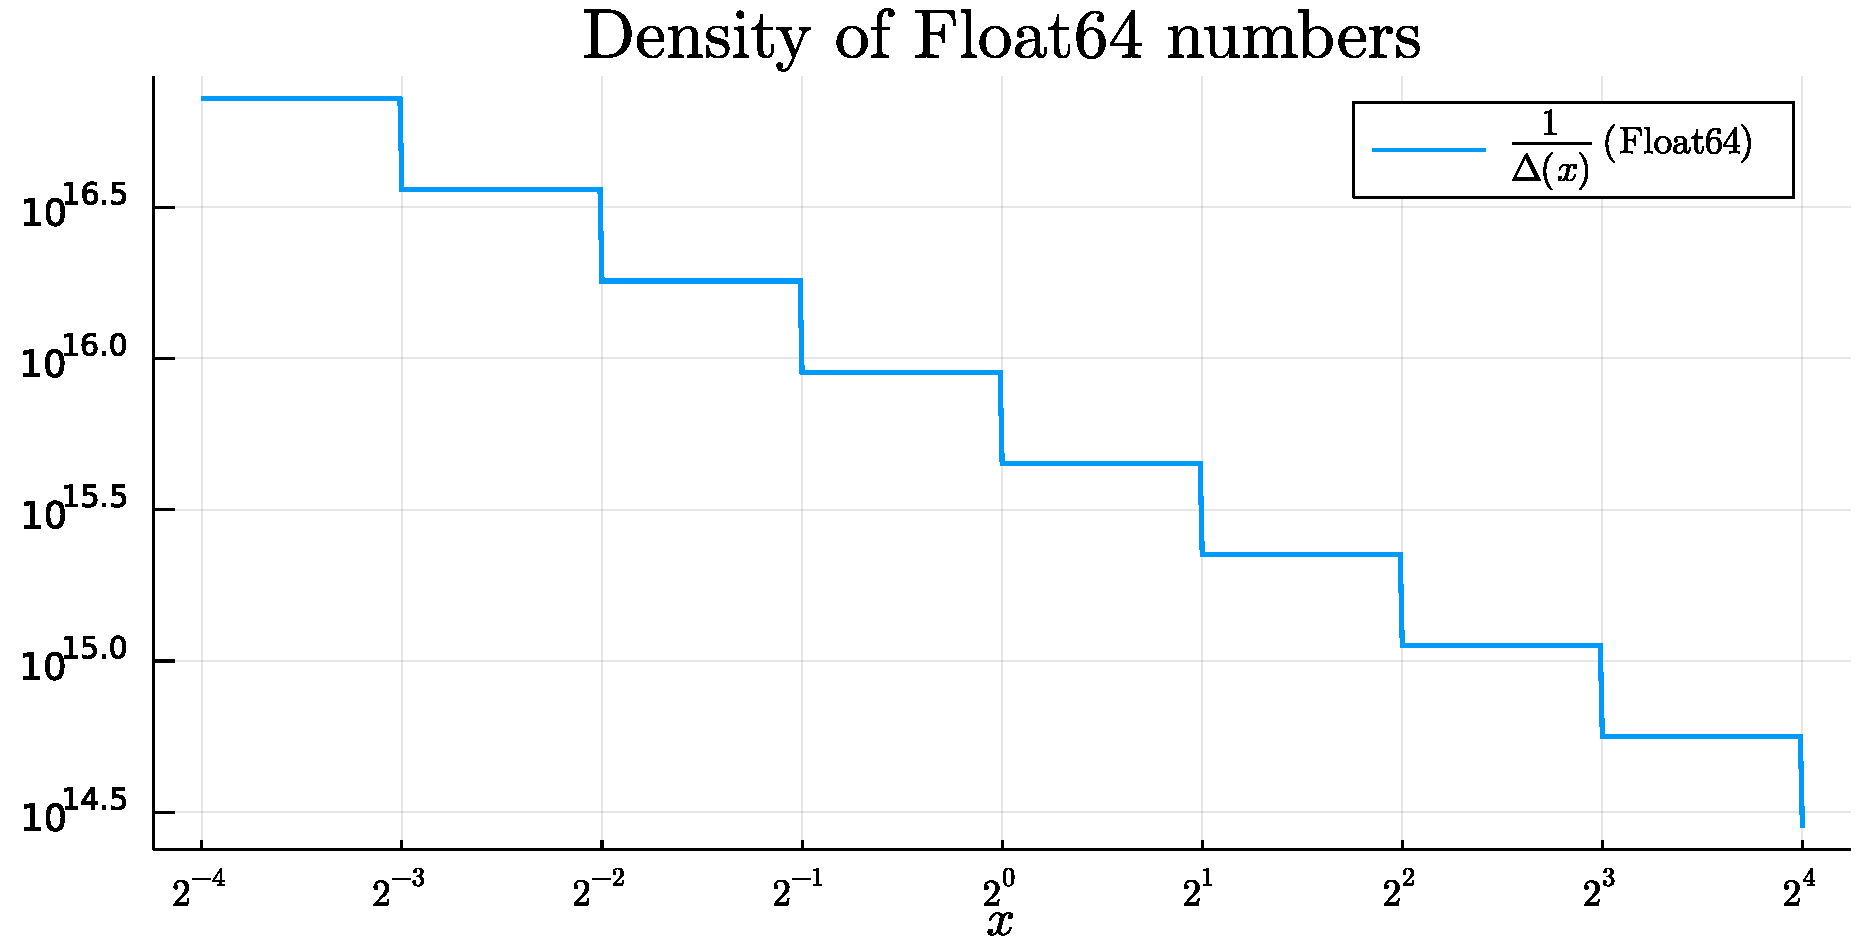
\includegraphics[width=.8\textwidth]{figures/float64_density.pdf}
    \caption{%
        Density of the double-precision floating point numbers,
        measured here as~$1/\Delta(x)$ where,
        for $x \in \floating_{64}$,
        $\Delta(x)$ denotes the distance between $x$ and its successor in $\floating_{64}$.
    }%
    \label{fig:float64_density}%
\end{figure}

\begin{figure}[ht]
    \centering
    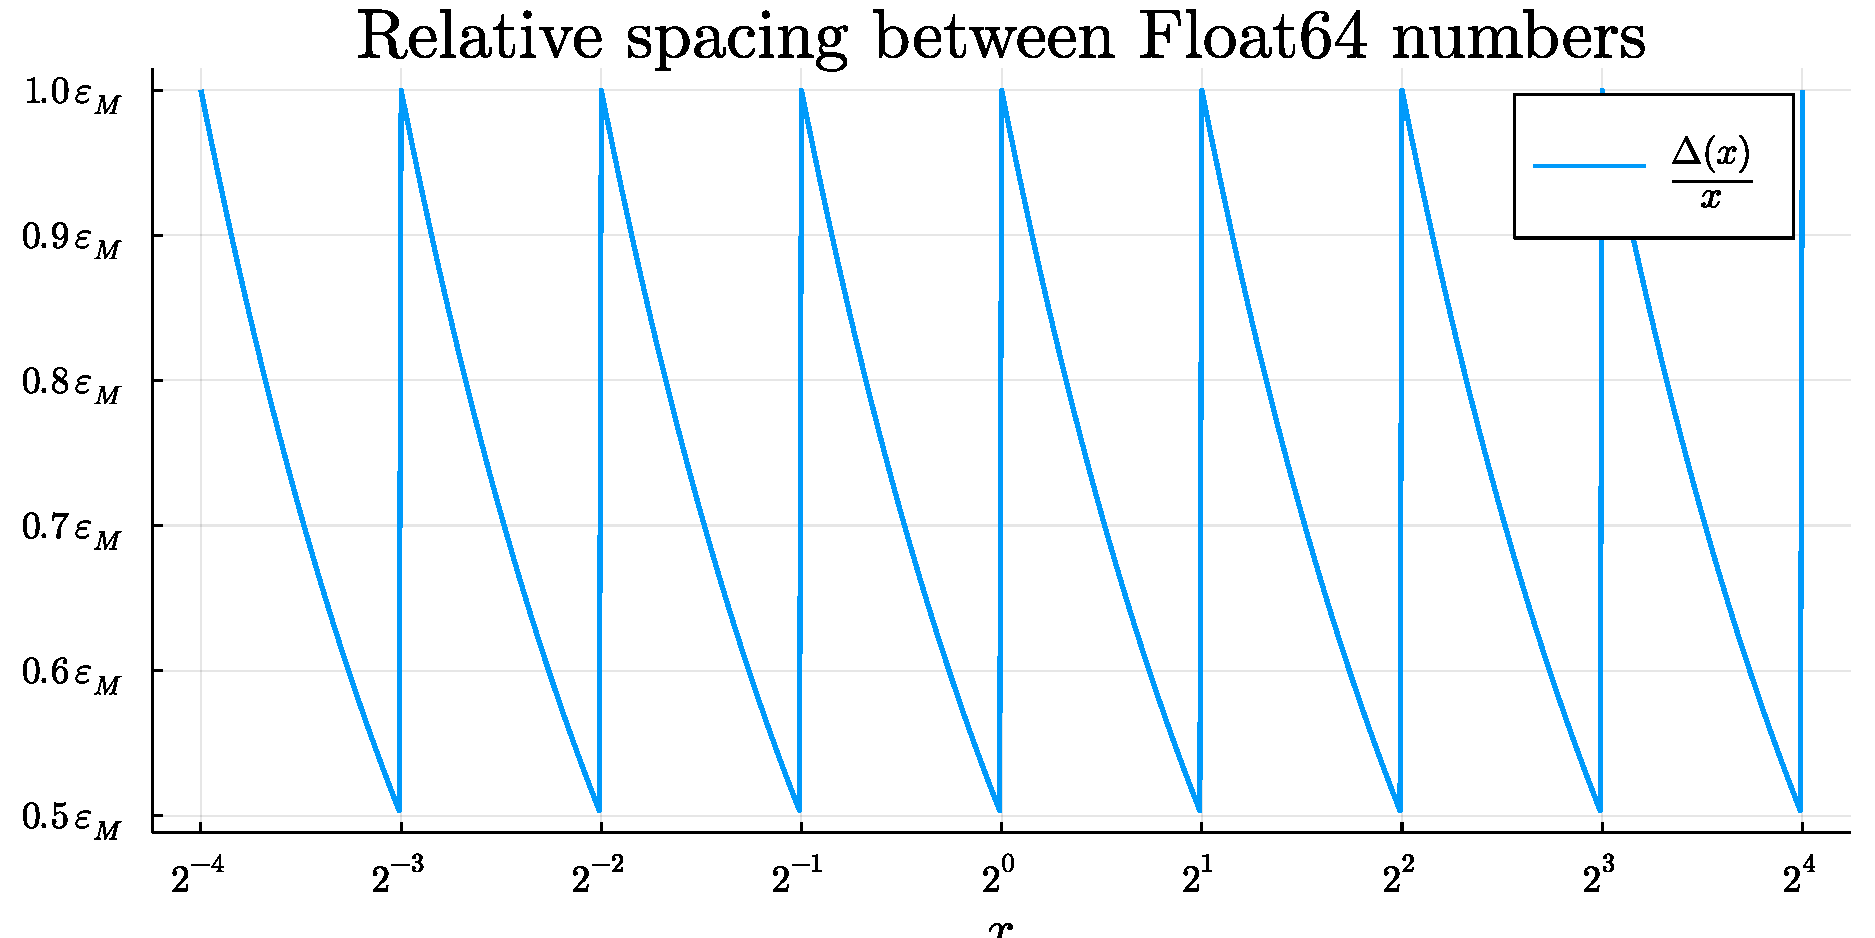
\includegraphics[width=.8\textwidth]{figures/float64_spacing.pdf}
    \caption{%
        Relative spacing between successive double-precision floating point numbers in the ``normal range''.
        The relative spacing oscillates between $\frac{1}{2} \varepsilon_M$ and $\varepsilon_M$.
    }%
    \label{fig:float64_spacing}
\end{figure}

The picture of the relative spacing between successive floating point numbers looks quite different for denormalized numbers.
This is illustrated in \cref{fig:float64_spacing_denormalized},
which shows that the relative spacing increases beyond the machine epsilon in the denormalized range.
Fortunately, in the usual $\floating_{32}$ and $\floating_{64}$ formats,
the transition between normalized and denormalized numbers occurs at such a small value that
rarely it needs worrying about.

\begin{figure}[ht]
    \centering
    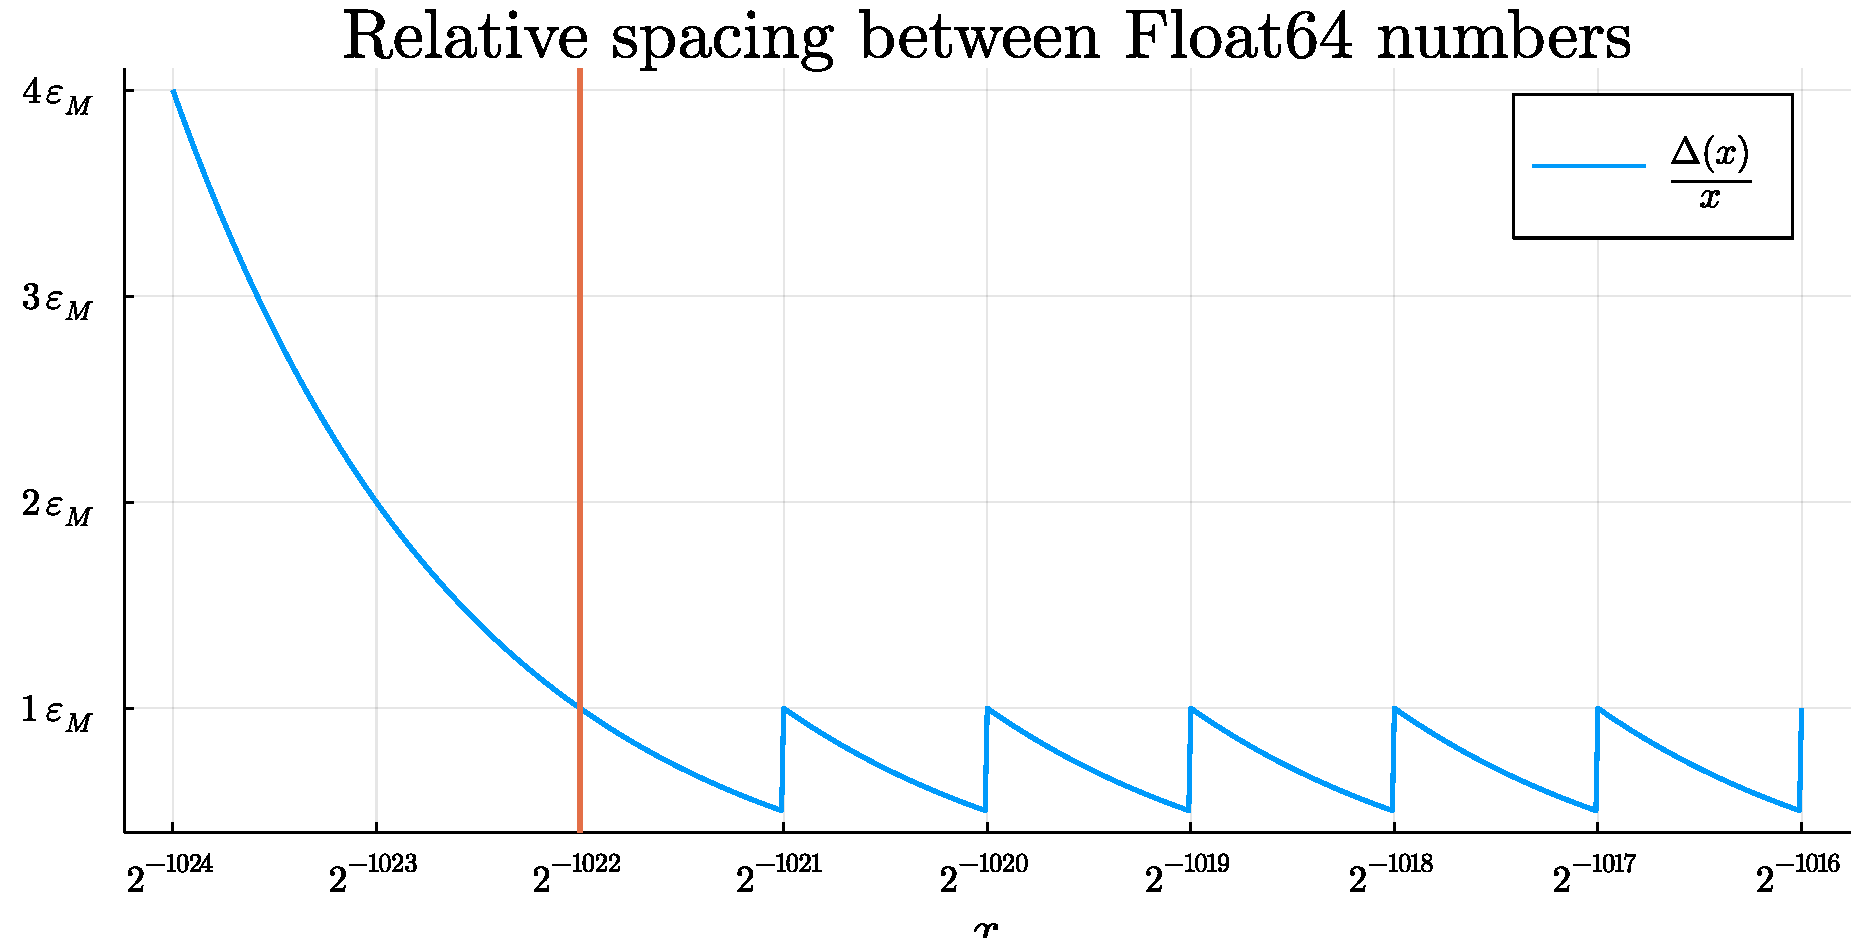
\includegraphics[width=.8\textwidth]{figures/float64_spacing_denormalized.pdf}
    \caption{%
        Relative spacing between successive double-precision floating point numbers,
        over a range which includes denormalized number.
        The vertical red line indicates the transition between denormalized and normalized numbers.
    }%
    \label{fig:float64_spacing_denormalized}
\end{figure}

\subsection{Exercises}%
\label{sub:exercises}

\begin{exercise}
    Write down the values of the smallest and largest, in absolute value,
    positive real numbers representable in the $\floating_{32}$ and $\floating_{64}$ formats.
\end{exercise}

\begin{exercise}
    [Relative error and machine epsilon]
    \label{exercise:machine_epsilon}
    Prove that the inequality~\eqref{eq:bound_epsilon_machine} is sharp.
\end{exercise}

\begin{exercise}
    [Cardinality of the set of floating point numbers]
    Show that, if $E_{\max} \geq E_{\min}$, then $\floating(p, E_{\min}, E_{\max})$ contains exactly
    \[
        (E_{\max} - E_{\min}) 2^{p} + 2^{p+1} - 1
    \]
    \emph{distinct real numbers}.
    (In particular, the special values \texttt{Inf}, \texttt{-Inf} and \texttt{NaN} are not counted.)
    \textbf{Hint:} Count first the normalized and then the denormalized numbers.
\end{exercise}

\section{Arithmetic operations between floating point formats}%
\label{sec:arithmetic_operations_between_floating_point_formats}

Now that we have presented the set of values representable on a computer,
we endeavour in this section to understand precisely how arithmetic operations between floating point formats are performed.
The key mechanism governing arithmetic operations on a computer is that of \emph{rounding},
the process by which an infinitely precise real number is approximated by a floating point number of the type presented in the previous section.
The IEEE 754 standard specifies several mechanisms for rounding numbers,
known as \emph{rounding modes}.
The default rounding mode is \emph{round to nearest},
which behaves as follows:
\begin{itemize}
    \item
        \textbf{Standard case}:
        An infinitely precise real number is rounded to the \emph{nearest representable number},
        if this number is unique.
    \item
        \textbf{Edge case}:
        When there are two equally near representable numbers in the floating point format,
        the one with the least significant bit equal to zero is delivered.
    \item
        \textbf{Infinities}:
        If the real number $x$ is larger than the largest representable number in the format,
        that is larger than or equal to $x_{\max} = 2^{E_{\max}} (2 - 2^{-p-1})$,
        then there are two cases,
        \begin{itemize}
            \item If $x < 2^{E_{\max}} (2 - 2^{-p})$, then $x_{\max}$ is delivered;
            \item Otherwise, the special value~\texttt{Inf} is delivered.
        \end{itemize}
        In other words, $x_{\max}$ is delivered if it would be delivered by following the rules of the first two bullet points
        in a different floating point format with the same precision but an exponent $E_{\max}$ larger by one.
        A similar rule applies for large negative numbers.
\end{itemize}

\begin{exercise}
    In the \texttt{Float16} format, explain why
    \begin{minted}{julia}
        Float16(1 + 2^-10 + 2^-11) == Float16(1 + 2^-10)
    \end{minted}
    evaluates to \texttt{false}
    but
    \begin{minted}{julia}
        Float16(1 + 2^-11) == Float16(1)
    \end{minted}
    evaluates to \texttt{true}.
\end{exercise}

When a binary arithmetic operation ($+$, $-$, $\times$, $/$) is performed on a computer,
the result delivered by the computer coincides is the exact result of the operation,
up to rounding according to the rules given above.
More precisely,
the arithmetic operation is performed as if the computer first calculated an intermediate exact result,
and then rounded this intermediate result in order to provide a final result in the appropriate floating point format.
The format of the end result,
known as the \emph{destination format},
depends on that of the arguments of the arithmetic operation:
as a rule of thumb,
the destination format is the most precise among the formats of the arguments.
\begin{example}
This can be readily verified in Julia using the \texttt{typeof} function.
\begin{minted}{julia}
julia> typeof(Float16(1) + Float32(1))
Float32

julia> typeof(Float32(1) + Float64(1))
Float64

julia> typeof(Float16(1) + Float64(1))
Float64
\end{minted}
\end{example}

If an mathematical expression contains several binary arithmetic operations to be performed in succession,
the floating point result of each intermediate calculation is stored in a floating point format dictated by the formats of its argument,
and this floating point number is employed in the next binary operation.
A consequence of this mechanism of arithmetic operations is that the operands $+$ and $*$ are generally not associative.
Consider for example the following \emph{Julia} expressions:
\begin{code}
    \captionof{listing}{Non-associativity of floating point addition}
    \label{code:non_associativity}
\begin{minted}{julia}
julia> (Float16(1) + Float16(2^-11)) + Float16(2^-11)
Float16(1.0)

julia> Float16(1) + (Float16(2^-11) + Float16(2^-11))
Float16(1.001)
\end{minted}
\end{code}
Can you explain this difference in behavior?
For the computer, each these expressions contains two binary additions,
with one involving the result of the other as an argument.
To explain this somewhat surprising result,
we begin by writing the binary representations of the floating point numbers in the $\floating_{16}$ representation.
\begin{align*}
    1 &= (-1)^0 \times 2^0 \times \texttt{1.0000000000} \\
    2^{-11} &= (-1)^0 \times 2^{-11} \times \texttt{1.0000000000}.
\end{align*}
In the first expression,
the addition \mintinline{julia}{Float16(1) + Float16(2^-11)} is first performed.
The exact result of this operation is $r = 1 + 2^{-11}$,
which in normalized binary notation is
\[
    r_2 = 1.\underbrace{0000000000}_{\text{10 zeros}}1.
\]
Since the length of the significand in the half-precision (\texttt{Float16}) format is only $p = 11$,
this number is not representable in $\floating_{16}$.
The result of the addition is therefore rounded to the member of $\floating_{16}$ nearest to $r$,
provided this is unique.
In this example, there are two members of~$\floating_{16}$ equally near~$r$,
which we denote by $\widehat r$ and $\widetilde r$:
\begin{align*}
    \widehat r_2 = 1.\underbrace{0000000000}_{\text{10 zeros}},
    \qquad
    \widetilde r_2 = 1.\underbrace{000000000}_{\text{9 zeros}}1.
\end{align*}
According to the standard,
the former is delivered, since its least significant bit is zero.
Therefore, the result of the addition \mintinline{julia}{Float16(1) + Float16(2^-11)}
is \mintinline{julia}{Float16(1)}.
In order to complete the evaluation of the first expression,
it remains to evaluate
\mintinline{julia}{Float16(1) + Float16(2^-11)},
which of course also evaluates to \mintinline{julia}{Float16(1)}.

In the second expression,
the first addition performed is \mintinline{julia}{Float16(2^{-11}) + Float16(2^-11)},
the exact result of which is representable in $\floating_{16}$.
The second addition that is performed is then \mintinline{julia}{Float16(1) + Float16(2^-10)},
which also results in a number representable in $\floating_{16}$.

\begin{remark}
To be complete,
one should explain why the result of the addition
in the second expression of~\cref{code:non_associativity},
equal to $1.0000000001$ in binary format and 1.0009765625 in decimal format,
is rendered as $1.001$ by Julia.
A detailed explanation would require a careful study of the rules specified in the standard regarding conversion between binary and decimal formats.
We content ourselves here with a couple remarks:
\begin{itemize}
    \item
        Although the string representation of the result given by Julia is only approximate,
        internally the value of the result is stored exactly:
        \begin{minted}{julia}
        julia> Float16(1 + 2^-10) == 1.0009765625
        true
        \end{minted}
    \item
        The relative precision of a number in $\floating_{16}$ is generally of the order of $2^{-(p-1)} = 2^{-10} \approx 10^{-3}$,
        except for subnormal numbers.
        By relative precision, we mean here the relative distance between a floating point number $x$
        and the one immediately succeeding it, which we denote by $x_{+}$.
        In fact, if $b_0 = 1$ and $x_{+} \neq \texttt{Inf}$,
        then this distance is equal to
        \[
            \frac{x_{+} - x}{x} = \frac{2^{-(p-1)}}{(1.b_1 b_2 \dots b_{p-2} b_{p-1})_2} \leq 2^{-(p-1)}.
        \]
        It is therefore not unreasonable that only 4 digits should be included (most of the time) in the decimal representation of half-precision numbers.

        The distance between adjacent floating point numbers is usually known as the \emph{machine epsilon},
        and it is accessible in Julia using the~\texttt{eps} function.
        For example, \mintinline{julia}{eps(Float64)} returns the machine epsilon for the \texttt{Float64} type,
        which is equal to approximately $2 \times 10^{-16}$.
\end{itemize}
\end{remark}



% For example,
% we endeavour in this section to understand precisely what happens when an operation of the form
% ``\texttt{a = 2.0 + 0.1 * 3.0}''
% is issued to the computer.

\section{Encoding of floating point numbers}%
\label{sec:encoding_of_floating_point_numbers}

Once a number format is specified through parameters $(p, E_{\min}, E_{\max})$,
the choice of encoding,
i.e.\ the machine representation of numbers in this format,
has no bearing on the magnitude and propagation of roundoff errors.
Studying encodings is, therefore, not essential for our purposes in this course,
but we opted to cover the topic anyway in the hope that this will help the students build intuition on floating point numbers.
The material in this section is for information purposes only.

We already mentioned, in~\cref{sec:set_of_values},
that the representation (sign, exponent and significand) of any nonzero number in a floating point format $\floating(p, E_{\min}, E_{\max})$ can be made unique.
In this section,
we discuss how these numbers are stored on the computer in practice.
As their names suggest, the \texttt{Float32} and \texttt{Float64} formats use 32 and 64 bits of memory, respectively.
A naive approach for encoding these number formats would be to store the full binary representations of the sign, exponent and significand.
For the \texttt{Float32} format,
this approach would requires 1 bit for the sign,
8 bits to cover the 254 possible values of the exponent, and 24 bits for the significand,
i.e.\ for storing $b_0, \dots, b_{p-1}$.
This leads to a total number of 33 bits,
which is one more than is available,
and this is without the special values \texttt{NaN}, \texttt{Inf} and \texttt{-Inf}.
So how are numbers in the $\floating_{32}$ and $\floating_{64}$ formats actually stored?
To answer this question,
we begin with two observations:
\begin{itemize}
    \item
        If $E > E_{\min}$,
        then necessarily $b_0 = 1$ in the unique representation of the significand.
        Consequently, the leading bit need not be explicitly specified in the case;
        in this case it is said to be \emph{implicit}.
        We will see that $p-1$ bits are in fact sufficient for the significand.
    \item
        In the $\floating_{32}$ format,
        8 bits are reserved for the exponent,
        which enable the representation of $2^8 = 256$ different values,
        but there are only 254 possible values for the exponent.
        This suggests that $256 - 254 = 2$ combinations of the 8 bits can be exploited in order to,
        for example, represent the special values \texttt{Inf}, \texttt{-Inf} and \texttt{NaN}.
\end{itemize}

Simplifying a bit,
we may view a single precision floating point number as an array of bits with indices 0 to 31:
\begin{center}
    \definecolor{lightcyan}{rgb}{0.84,1,1}
    \definecolor{lightgreen}{rgb}{0.64,1,0.71}
    \definecolor{lightred}{rgb}{1,0.7,0.71}
    \begin{bytefield}[bitheight=\widthof{~Sign~}, boxformatting={\centering\small}]{32}
        \bitheader[endianness=little]{0, 8, 31} \\
        \bitbox{1}[bgcolor=lightcyan]{\rotatebox{90}{Sign}} &
        \bitbox{8}[bgcolor=lightgreen]{Encoded exponent} &
        \bitbox{23}[bgcolor=lightred]{Encoded significand}
    \end{bytefield}
\end{center}
According to the IEEE 754 standard,
the first bit is the sign $s$,
the next 8 bits $e_0 e_1 \dots e_6 e_7$ encode the exponent,
and the last 23 bits $b_1 b_2 \dots b_{p-2} b_{p-1}$ encode the significand.
Let us introduce the integer number $e = (e_0 e_1 \dots e_6 e_7)_2$;
that is to say, $0 \leq e \leq 2^8 -1$ is the integer number whose binary representation
is given by $e_0 e_1 \dots e_6 e_7$.
One may determine the exponent and significand of a floating point number from the following rules.
\begin{itemize}
    \item
        \textbf{Subnormal numbers}:
        If $e = 0$, then the implicit leading bit $b_0$ is zero,
        the fraction is $b_1 b_2 \dots b_{p-2} b_{p-1}$, and the exponent is $E = E_{\min}$.
        In the format of~\cref{sec:set_of_values},
        one may write $x = (-1)^s 2^{E_{\min}} 0.b_1b_2 \dots b_{p-2} b_{p-1}$.
        In particular, if $b_1 b_2 \dots b_{p-2} b_{p-1} = 00\dots00$,
        then it holds that $x = 0$.
    \item
        \textbf{Normalized numbers}:
        If $0 < e < 255$,
        then the implicit leading bit $b_0$ of the significand is $1$
        and the fraction is given by $b_1 b_2 \dots b_{p-2} b_{p-1}$.
        The exponent is given by
        \[
            E = e - \mathrm{bias} = E_{\min} + e - 1.
        \]
        where the exponent bias for the single and double precision formats are given in~\cref{table:floating_point_formats_encoding}.
        In this case $x = (-1)^s 2^{e - \mathrm{bias}} 1.b_1b_2 \dots b_{p-2} b_{p-1}$.
        Notice that $E = E_{\min}$ if $e = 1$,
        as in the case of subnormal numbers.
    \item
        \textbf{Infinities}:
        If $e = 255$ and $b_1 b_2 \dots b_{p-2} b_{p-1} = 00\dots00$,
        then $x = (-1)^s \texttt{Inf}$.
    \item
        \textbf{Not a Number}:
        If $e = 255$ and  $b_1 b_2 \dots b_{p-2} b_{p-1} \neq 00\dots00$,
        then $x = \texttt{NaN}$.
        Notice in particular that the special value \texttt{NaN} can be encoded in many different manners.
        These extra degrees of freedom were reserved for passing information on the reason for the occurrence of $\texttt{NaN}$,
        which is usually an indication that something has gone wrong in the calculation.
\end{itemize}

\begin{table}[hb]
    \centering
    \begin{tabular}{|c|c|c|c|}
        \hline
        & Half precision & Single precision & Double precision
        \\ \hline
        Exponent bias ($-E_{\min} + 1$) & $15$ & $127$ & $1023$
        \\ \hline
        Exponent encoding (bits) & 5 & 8 & 11
        \\ \hline
        Significand encoding (bits) & 10 & 23 & 52
        \\ \hline
    \end{tabular}
    \caption{Encoding parameters for floating point formats}%
    \label{table:floating_point_formats_encoding}
\end{table}

\begin{exercise}
    Determine the encoding of the \texttt{Float32} numbers:
    \begin{itemize}
        \item $x = 2.0^{E_{\min}}$.
        \item $x = - 2.0^{E_{\min} - p - 1} = - 2.0^{-149}$
        \item $x = 2.0^{E_{\max}} (2-2^{-p+1})$
    \end{itemize}
    Check your results using the Julia function \texttt{bitstring}.
\end{exercise}

\section{An example: numerical differentiation}%
To illustrate this point,
consider the following program for calculating the derivative of the function $f(x) = \log(x)$ at $x = 1$.
\[
    f'(x) \approx \frac{\log(x + \varepsilon) - \log(x)}{\varepsilon}
\]
\begin{minted}{julia}
f(x) = log(x)
x + δ
for i in 1:10
end
abcdefghijklmnopqr
\end{minted}

\begin{exercise}
    [Avoiding overflow]
    Write a code to calculate the weighted average
    \[
        S := \frac
        {\sum_{x=0}^{L} \e^x x}
        {\sum_{x=0}^{L} \e^x},
        \qquad L = 1000.
    \]
\end{exercise}



% \begin{exercise}
%     Show that $31_{8} = 25_{10}$,
%     an equation sometimes written as~${\rm Oct} 31 = {\rm Dec} 25$.
% \end{exercise}

% \begin{example}
%     In the HTML language,
%     colors are represented by strings of the type $\texttt{\#rrggbb}$.
% \end{example}

% \begin{example}
%     [Computation of the standard deviation]
% \end{example}

% \begin{example}
%     [Calculation of the derivative]
%     A classic π example of cancellation is when calculating derivatives.
%     Consider the following approximation of $\frac{\d}{\d x}\log(x) \vert_{x=1}$:
%     \[
%         	\frac{\log(x + \varepsilon) - \log(x)}{\varepsilon}
%     \]
% \end{example}

% \begin{example}
%     [Second-degree equation]
%     Consider the equation
%     \[
%         x^2 - \varepsilon x + 1 = 0
%     \]
% \end{example}

% \begin{theorem}
%     {Title of theorem}
%     \label{thm:test}
%     hello
% \end{theorem}

% \begin{example}
%     [A test example]
%     hello
% \end{example}

% \begin{lemma}
%     [Title of the lemma]
%     {Title of theorem}
%     \label{lemma:test}
%     hello
% \end{lemma}

% \begin{remark}
%     [Hello]
%     test
% \end{remark}

% \begin{theorem}
%     {Title of theorem}
%     test
% \end{theorem}

% \cref{lemma:test}

\section{Discussion and supplemental reading}%
\label{sec:discussion_and_bibliograhpy}
This chapter is mostly based on the original 1985 IEEE 754 standard~\cite{ieee754} and the reference book~\cite{MR2265914}.
A~significant revision to the 1985 IEEE standard was published in 2008~\cite{ieee2008},
adding for example specifications for the half precision and quad precision formats,
and a minor revision was published in 2019~\cite{ieee2019}.
The original IEEE standard and its revisions constitute the authoritative guide on floating point formats.
It was intended to be widely disseminated and is written very clearly and concisely,
but is not available for free online.
Another excellent source for learning about floating point numbers and roundoff errors is D.\ Goldberg's~paper ``\emph{What every computer scientist should know about floating-point arithmetic}''~\cite{goldberg1991every},
freely available online.

\section{Exercises}%
\label{sec:exercises}

\begin{exercise}
    [Calculating the sample variance]
    Assume that $(x_n)_{1 \leq n \leq n}$ are independent random variables distributed according to
    the uniform distribution $\mathcal U(L, L+1)$.
    That is, each~$x_n$ takes a random value uniformly distributed between $L$ and $L+1$.
    In Julia, these samples can be generated with the following lines of code:
    \begin{minted}{julia}
        N, L = 10^9, 10^9
        x = L .+ rand(N)
    \end{minted}
    It is well know that the variance of $x_n \in \mathcal U(L, L+1)$ is given by~$\sigma^2 = \frac{1}{12}$.
    Numerically, the variance can be estimated from the \emph{sample variance}:
    \begin{equation}
        \label{eq:sample_variance_1}
        s^2 = \frac{1}{N-1} \sum_{n=1}^{N} (x_n - \bar x)^2,
        \qquad \bar x = \frac{1}{N} x_n.
    \end{equation}
    The sample variance may also be written as
    \begin{equation}
        \label{eq:sample_variance_2}
        s^2 = \frac{1}{N-1} \left(\left(\sum_{n=1}^{N} x_n^2\right) - N \bar x^2 \right).
    \end{equation}
    Implement both~\eqref{eq:sample_variance_1} and~\eqref{eq:sample_variance_2}
    and compare the accuracy of the result.
    In order to estimate the true value of $s^2$,
    use the \texttt{BigFloat} format.
\end{exercise}


% In this chapters,
% we covered the fundamentals of floating point arithmetics,
